% \section{Motivation}
% \begin{frame}[c]{The Need for 3D Deep Learning}
%     \large
%     \begin{figure}
    \captionsetup[subfigure]{labelformat=empty}
    \begin{subfigure}{0.3\textwidth}
        % lidar car visualization
        Robot Perception \\
        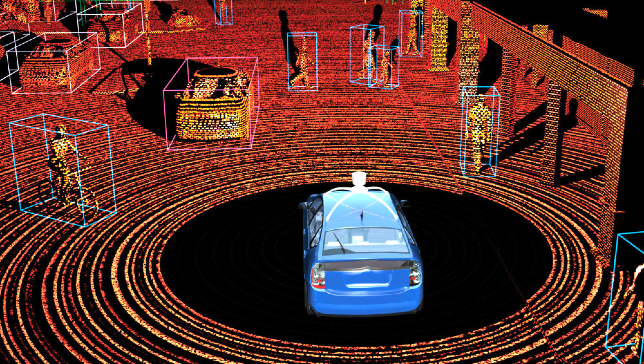
\includegraphics[height=0.35\textheight]{p02_6}
        \caption{source: Scott J Grunewald}
    \end{subfigure}
    \hspace{5mm}
    \begin{subfigure}{0.3\textwidth}
        % phone AR
        Augmented Reality \\
        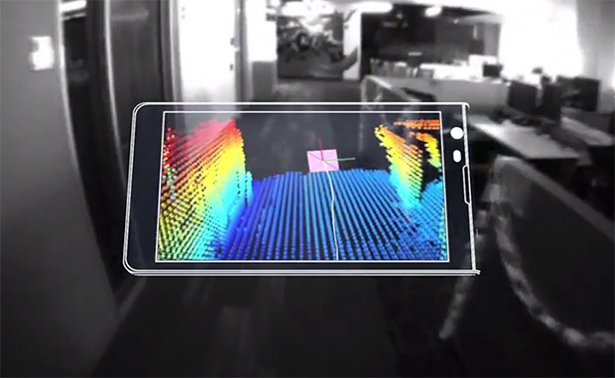
\includegraphics[height=0.35\textheight]{p02_8}
        \caption{source: Google Tango}
    \end{subfigure}
    \hspace{2mm}
    \begin{subfigure}{0.3\textwidth}
        % solidworks 3D objects
        Shape Design \\
        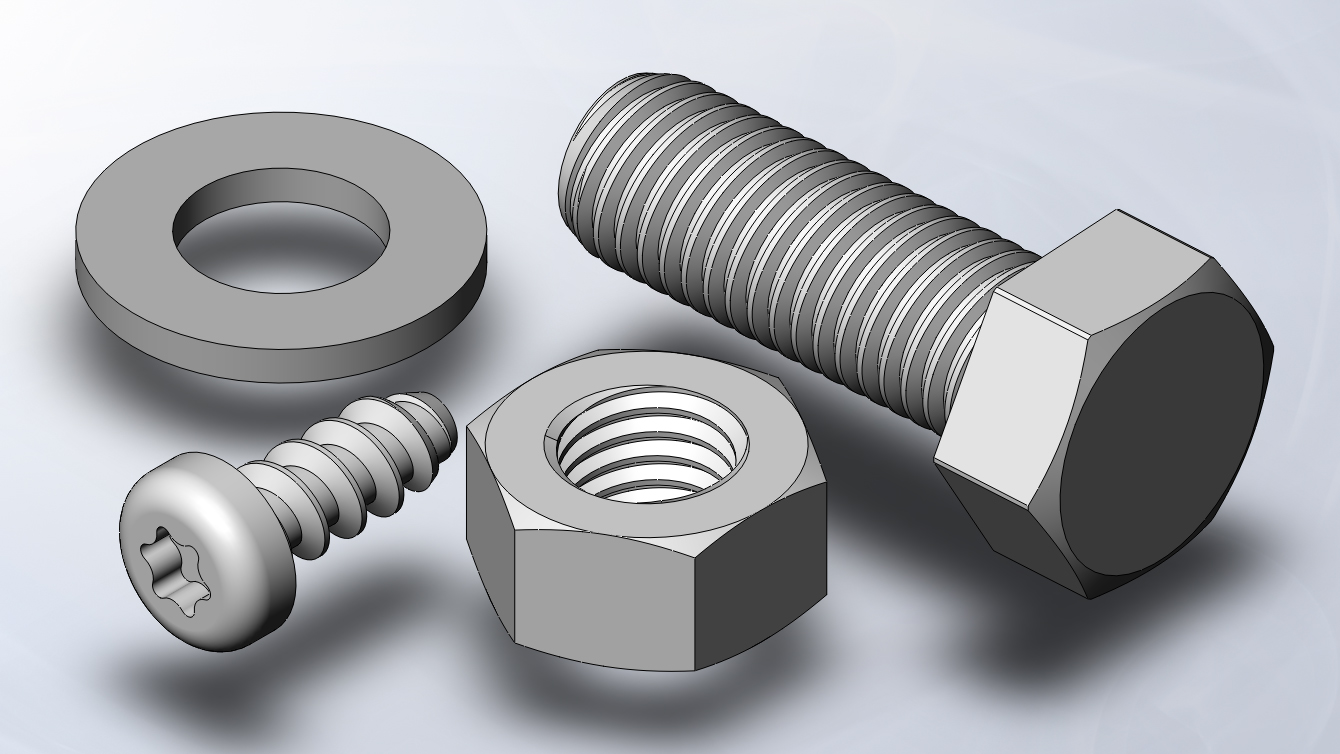
\includegraphics[height=0.35\textheight]{p02_7}
        \caption{source: solidworks}
    \end{subfigure}
    \blfootnote{Figures and captions from CVPR presentation to \cite{qi2017pointnet}.}
\end{figure}

%     \Large
%     \vspace{1em}
%     A number of emerging 3D applications shape the need for 3D deep learning.
%     \pnote{
%         Es entstehen viele Anwendungen die Wahrnehmung  \\
%         oder Interaktion in 3D benötigen.
%         \par
%         - viele Anwendungen im 3D bereich entstehen \\
%         - brauchen Wahrnehmung oder Interaktion in 3D \\
%         - um diese zu bedienen: hoher bedarf \\
%         - spezifisch auf 3D zugeschnitten \\
%         - Erster: PointNet \\
%     }
% \end{frame}


\section{Representation}
\begin{frame}[c]{Common Representations of 3D Data}
    \begin{figure}
    % \captionsetup[subfigure]{labelformat=empty, size=\large, labelfont={black, bf}}
    \captionsetup[subfigure]{labelformat=empty, font={large, color=black}}
    \begin{subfigure}{0.23\textwidth}
        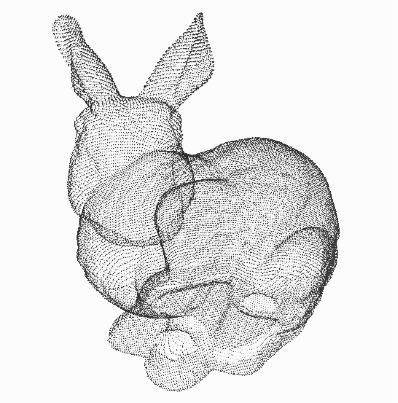
\includegraphics[height=0.35\textheight]{p04_12}
        \caption{Point Cloud}
    \end{subfigure}
    \begin{subfigure}{0.23\textwidth}
        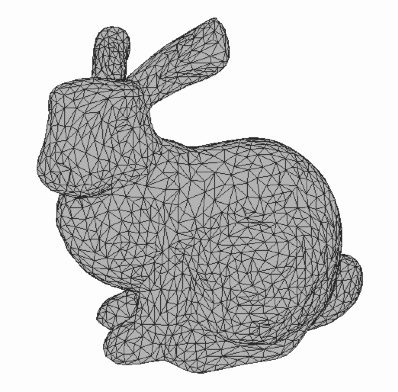
\includegraphics[height=0.35\textheight]{p04_13}
        \caption{Mesh}
    \end{subfigure}
    \begin{subfigure}{0.23\textwidth}
        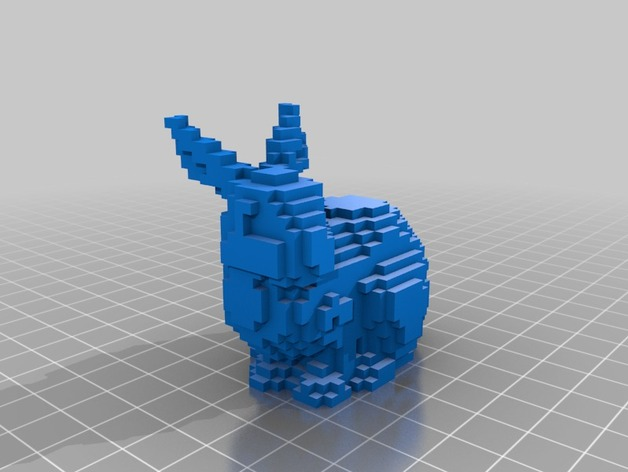
\includegraphics[height=0.35\textheight]{p04_14}
        \caption{Volumetric}
    \end{subfigure}
    \hspace{1mm}
    \begin{subfigure}{0.23\textwidth}
        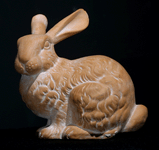
\includegraphics[height=0.35\textheight]{p04_15}
        \caption{View Rendering}
    \end{subfigure}
    \blfootnote{Figures and captions (partially) from CVPR presentation to \cite{qi2017pointnet}.}
\end{figure}

    \Large
    \vspace{1em}
    Contrary to 2D, 3D has many different popular representations.
    \pnote{Auszug an Beispielen}
\end{frame}


\begin{frame}[c]{Canonical Representation: Point Cloud}
    \large
    \begin{columns}
        \column{0.32\textwidth}
        \begin{itemize}
            \item Point cloud is close to \textbf{raw depth sensor data}
            \item Point cloud is \textbf{canonical} (easy conversion from and to other representations)
        \end{itemize}
        \color{ocre}
        \normalsize
        \vspace{2em}
        Individual figures from CVPR presentation to \cite{qi2017pointnet}
        \column{0.68\textwidth}
        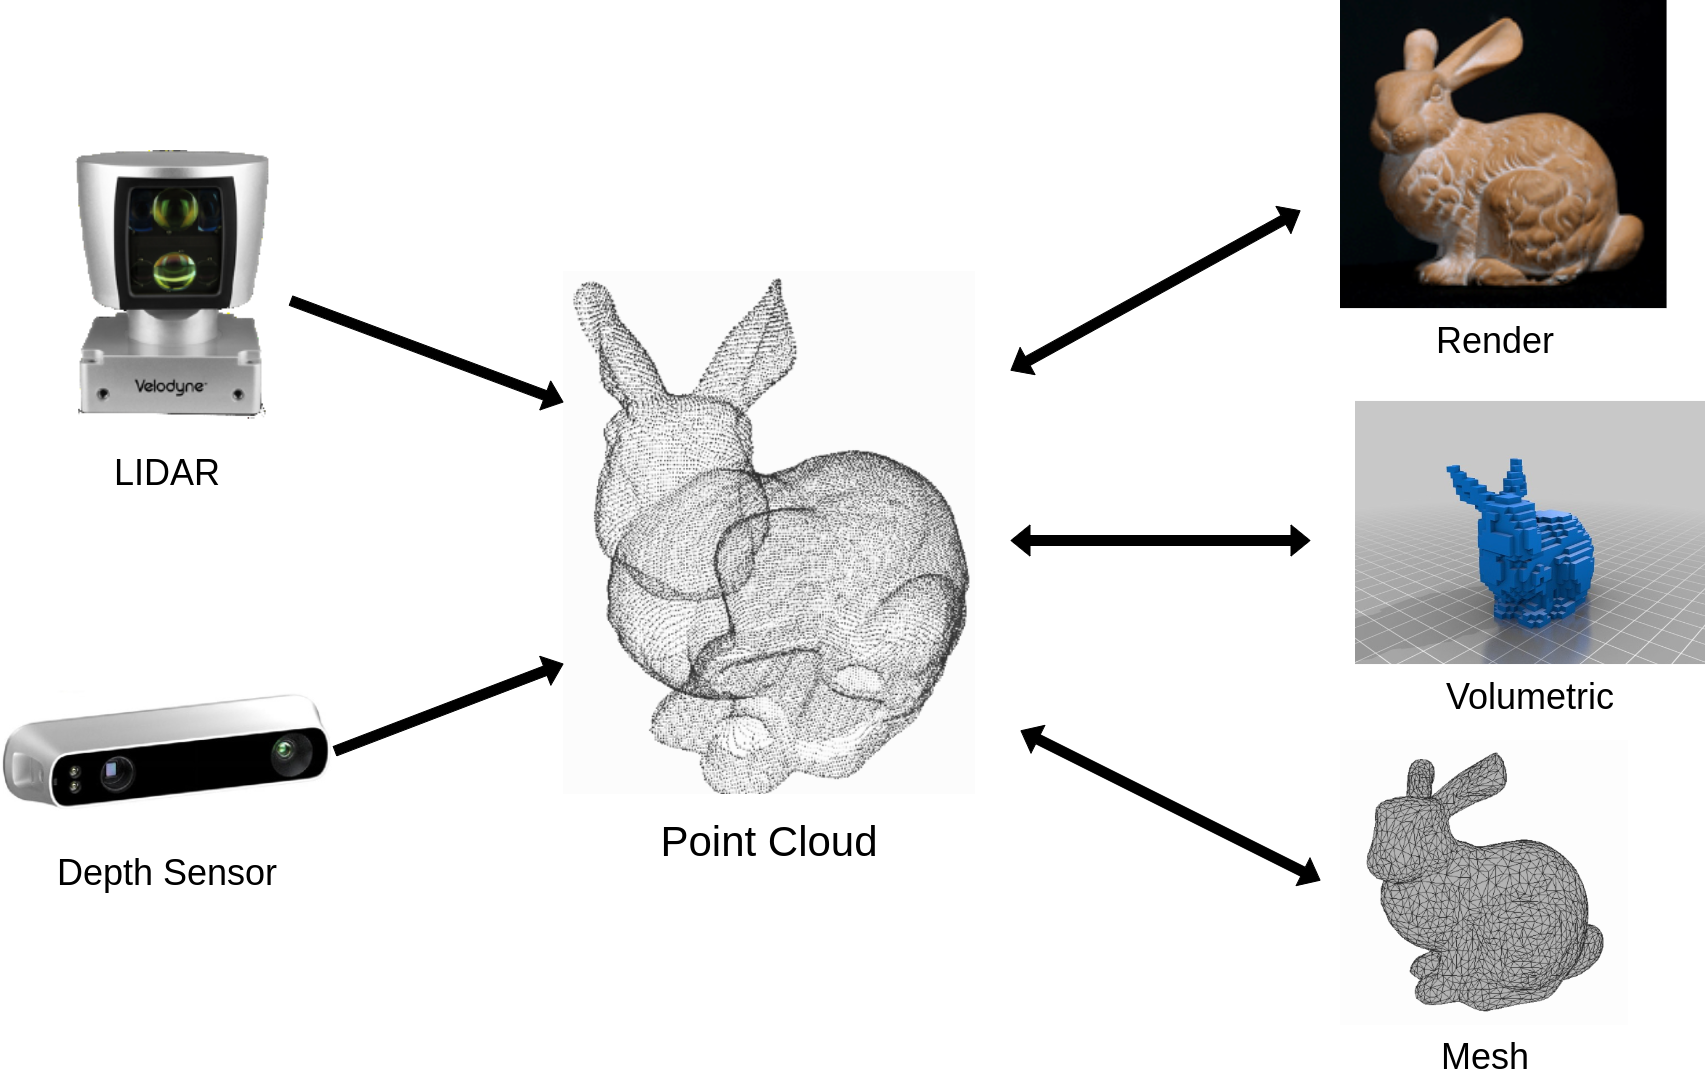
\includegraphics[height=0.75\textheight]{canonical}
    \end{columns}
    \pnote{
        - Am nächsten zu ursprünglichen Tiefendaten\\
        - Kanonische Form: andere lassen sich einfach umwandeln \\
        Allerdings: wenig Arbeit zu Point Cloud Features
    }
\end{frame}

